\documentclass{bmvc2k}

% \usepackage{algpseudocode}

\usepackage{algorithm}
\usepackage{algpseudocode}
\usepackage{ifthen}
%% Enter your paper number here for the review copy
% \bmvcreviewcopy{??}

\title{Image filtering and Hybrid images}

% Enter the paper's authors in order
% \addauthor{Name}{email/homepage}{INSTITUTION_CODE}
\addauthor{Taneesh \\2018csb1186}{}{1}

% Enter the institutions
% \addinstitution{Name\\Address}
\addinstitution{
 Indian Institute of Technology \\ Ropar
}

\runninghead{CS518 Computer Vision}{Assignment 1}

% Any macro definitions you would like to include
% These are not defined in the style file, because they don't begin
% with \bmva, so they might conflict with the user's own macros.
% The \bmvaOneDot macro adds a full stop unless there is one in the
% text already.
\def\eg{\emph{e.g}\bmvaOneDot}
\def\Eg{\emph{E.g}\bmvaOneDot}
\def\etal{\emph{et al}\bmvaOneDot}

%-------------------------------------------------------------------------
% Document starts here
\begin{document}

\maketitle

\begin{abstract}
Here I present the detailed report of assignment 1 of course CS518, Computer Vision where instead of using built in image filters
we are implementing correlation filters ourselves which can deal with grayscale as well as color images. 
Using this correlation filtering algorithm we are creating hybrid images which is a simplified version of SIGGRAPH 2006 paper by 
Oliva, Torralba, and Schyns~\cite{hybrid}.
\end{abstract}

%-------------------------------------------------------------------------
\section{Introduction}
\label{sec:intro}

The first part of the assignment is implementing how to filter an image if we are given an image and a filter in matrix form, we did not use filters provided by different libraries but implemented our own filter
which just correlated each part of the image with the filter progressively and then stores the new values in some other array which makes our new image. 

Given the fitler applier is ready now we have to use this to generate hybrid images. 


\textbf{The key idea:::}

If we are near an image then low frequencies are visible and when we are away from image high
frequencies are prominently visible. 

So if we can add two different images (which are kind of similar in some features like cat and dog or fist or submarine etc.) one with high frequencies and other with low frequencies then we can get an hybrid image 
which will show something else when nearby and some other thing when far away. 

So here we implement  \emph{my\_imfilter(image, filter)} function to filter out an image given the filter. 

We first test it with some filters provided in proj1\_test\_filtering.py

After that we use this filtering function to correlate a gaussian and our images. 

From there we find low frequencies and high frequencies. 

Add these frequencies and save our images. 

To visualize downscaling has been done which lets us to observe if the image is really hybrid.

Other functions used are normalize(image) as we were applying operations on images the values of the images were going out of bound, and this was causing an error 
to reslove the error we normalize the image, in other words map the image again to (0 to 1) in float.

Unlike matlab we did not have fspecial(gaussian) so we implemented our own gaussian\_filter(shape, sigma) function which returns a float gaussian array. 




%-------------------------------------------------------------------------
\section{Methodology}
\label{sec:Methodology}
We first show the implementation of the my\_imfilter(image, filter) function.

In order to implement \emph{my\_imfilter(image, filter)}, we just correlate our given image matrix with the given filter which is just point wise multipication of the filter and each submatrix in the image for each pixel and then we store the sum of all the values of the matrix thus obtained and set the value of the output image's pixel as this one. 


There is a bit of glitch here at boundaries as filter will definitely go out of bounds as when it goes to boundary or near boundary pixels so we have to pad our image matrix with appropriate number of zeroes so that when filter gets out of boundaries the values of zeroes gets multiplied. 

Below is step wise approach in words form. 

(1) First check if the dimensions of filter are both odd, else show error and return. 

(2) Now initialize the output array in code it's filtered\_image by copying the given image. 

(3) The number rows to be padded on front and back are number of rows of filter divided by 2 as integer and similarly for columns. 
Hence we get the new dimension of padded array. 

(4) Now check if the image is grayscale or rgb. 

  If image is rgb then we will intialize a 3d padded\_array else a 2d padded\_array.

 Initialize the padded matrix and put the image in centre of it. 

(3) Initialize an empty array of size same as image, Run the correlation/convolution (here correlation is done) algorithm on the image with the help of filter given. For each pixel point-wise multiply the subarray of size equal to filter's size with the filter get the sum and put the value of pixel in output as this sum. 

(4) Finally return the output array which is our 

Let's see some of the outputs our my\_imfilter(image,filter)

\begin{figure}[h!]
  \centering
  \begin{subfigure}[b]{0.3\linewidth}
    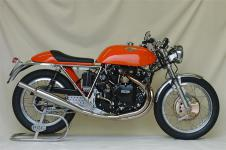
\includegraphics[width=\linewidth]{images/identity_image.jpg}
    \caption{Identity Image}
  \end{subfigure}
  \begin{subfigure}[b]{0.3\linewidth}
    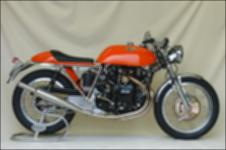
\includegraphics[width=\linewidth]{images/blur_image.jpg}
    \caption{Blurred Image}
  \end{subfigure}
  \begin{subfigure}[b]{0.3\linewidth}
    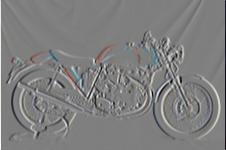
\includegraphics[width=\linewidth]{images/sobel_image.jpg}
    \caption{Sobel Image}
  \end{subfigure}
  \begin{subfigure}[b]{0.3\linewidth}
    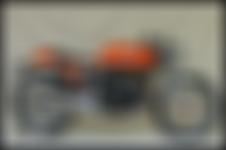
\includegraphics[width=\linewidth]{images/large_blur_image.jpg}
    \caption{Large Blur Image}
  \end{subfigure}
  \begin{subfigure}[b]{0.3\linewidth}
    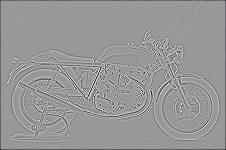
\includegraphics[width=\linewidth]{images/laplacian_image.jpg}
    \caption{Laplacian Image}
  \end{subfigure}
  \begin{subfigure}[b]{0.3\linewidth}
    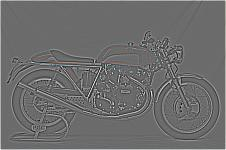
\includegraphics[width=\linewidth]{images/high_pass_image.jpg}
    \caption{High Pass Image}
  \end{subfigure}
  \caption{Different images obtained via proj1\_test\_filtering.py}
  \label{fig:coffee}
\end{figure}

% --------------------------------------------------------------------------

\begin{algorithm}[H]
	\caption {my\_imfilter(img, imfilter)}
   \begin{algorithmic}[1]

    \If{$ filter.width \%2 ==1 and  filter.length \%2 ==1 $}
      
        \State $ output \gets img.copy() $
        \State $ padding\_horizontal \gets (filter\_length -1 )/2 $
      \State $ padding\_vertical \gets (filter\_width -1)/2 $
      \If{$ img is grayscale $}
      \State $ final\_shape \gets (img\_length + 2*pad\_length, img\_width + 2*pad\_width)$
      \State $  padded\_array \gets matrix\_of\_zeroes(shape=final\_shape)  $
      \State $  padded\_matrix[pad\_length : img\_length + pad\_length, pad\_width : img\_width + pad\_width] \gets img  $
      
        \For {$  i \gets0:img\_length  $}
          \For{$  j\gets0:img\_width  $}
            \State {$ mult\_mat \gets mat\_mult(padded\_matrix[i:i+fil\_length, j:j+fil\_width], imfilter) $}
            \State {$  output[i,j] \gets sum\_matrix(mult\_mat)  $} 
          \EndFor
        \EndFor
      

      \Else

      \State $ final\_shape \gets (img\_length + 2*pad\_length, img\_width + 2*pad\_width, num\_ch)$
      \State $  padded\_array \gets matrix\_of\_zeroes(shape=final\_shape)  $
      \State $  padded\_matrix[pad\_length : img\_length + pad\_length, pad\_width : img\_width + pad\_width] \gets img  $
      \For {$  k \gets 0:img\_channels   $}
        \For {$  i \gets0:img\_length  $}
          \For{$  j\gets0:img\_width  $}
            \State {$ mult\_mat \gets mat\_mult(padded\_matrix[i:i+fil\_length, j:j+fil\_width, k], imfilter) $}
            \State {$  output[i,j,k] \gets sum\_matrix(mult\_mat)  $} 
          \EndFor
        \EndFor
      \EndFor
        \EndIf
      \State {\textbf{return} output}

      \Else 
      \State {$ return error $}
    
      
      \EndIf

    
    

  \end{algorithmic}
  

\end{algorithm}




\begin{algorithm}[H]
	\caption {for creating hybrid images}
   \begin{algorithmic}[1]

    \If{$ filter.width \%2 ==1 and  filter.length \%2 ==1 $}
      
        \State $ output \gets img.copy() $
        \State $ padding\_horizontal \gets (filter\_length -1 )/2 $
      \State $ padding\_vertical \gets (filter\_width -1)/2 $
      \If{$ img is grayscale $}
      \State $ final\_shape \gets (img\_length + 2*pad\_length, img\_width + 2*pad\_width)$
      \State $  padded\_array \gets matrix\_of\_zeroes(shape=final\_shape)  $
      \State $  padded\_matrix[pad\_length : img\_length + pad\_length, pad\_width : img\_width + pad\_width] \gets img  $
      
        \For {$  i \gets0:img\_length  $}
          \For{$  j\gets0:img\_width  $}
            \State {$ mult\_mat \gets mat\_mult(padded\_matrix[i:i+fil\_length, j:j+fil\_width], imfilter) $}
            \State {$  output[i,j] \gets sum\_matrix(mult\_mat)  $} 
          \EndFor
        \EndFor
      

      \Else

      \State $ final\_shape \gets (img\_length + 2*pad\_length, img\_width + 2*pad\_width, num\_ch)$
      \State $  padded\_array \gets matrix\_of\_zeroes(shape=final\_shape)  $
      \State $  padded\_matrix[pad\_length : img\_length + pad\_length, pad\_width : img\_width + pad\_width] \gets img  $
      \For {$  k \gets 0:img\_channels   $}
        \For {$  i \gets0:img\_length  $}
          \For{$  j\gets0:img\_width  $}
            \State {$ mult\_mat \gets mat\_mult(padded\_matrix[i:i+fil\_length, j:j+fil\_width, k], imfilter) $}
            \State {$  output[i,j,k] \gets sum\_matrix(mult\_mat)  $} 
          \EndFor
        \EndFor
      \EndFor
        \EndIf
      \State {\textbf{return} output}

      \Else 
      \State {$ return error $}
    
      
      \EndIf

    
    

  \end{algorithmic}
  

\end{algorithm}

%-------------------------------------------------------------------------
\section{Results and Observations}
\label{sec:Results}

Following are differen hybrid images obtained from the algorithm. 

\begin{figure}[h!]
  \centering
  \begin{subfigure}[b]{0.2\linewidth}
    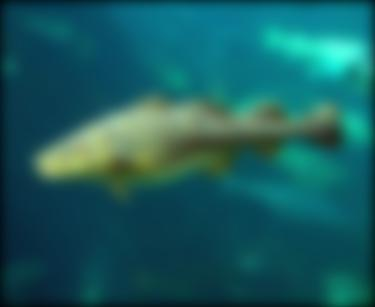
\includegraphics[width=\linewidth]{images/Fish_Sub/low_frequencies_fish_submarine.jpg}
     \caption{Low Freq}
  \end{subfigure}
  \begin{subfigure}[b]{0.2\linewidth}
    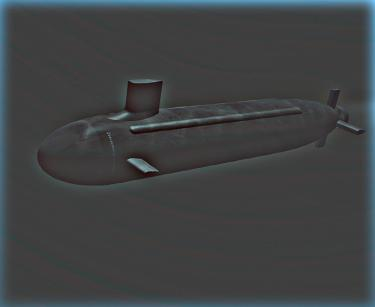
\includegraphics[width=\linewidth]{images/Fish_Sub/high_frequencies_fish_submarine.jpg}
    \caption{High Freq}
  \end{subfigure}
  \begin{subfigure}[b]{0.2\linewidth}
    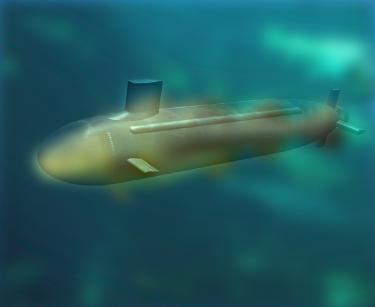
\includegraphics[width=\linewidth]{images/Fish_Sub/hybrid_image_fish_submarine.jpg}
    \caption{Hybrid Image}
  \end{subfigure}
  \begin{subfigure}[b]{0.5\linewidth}
    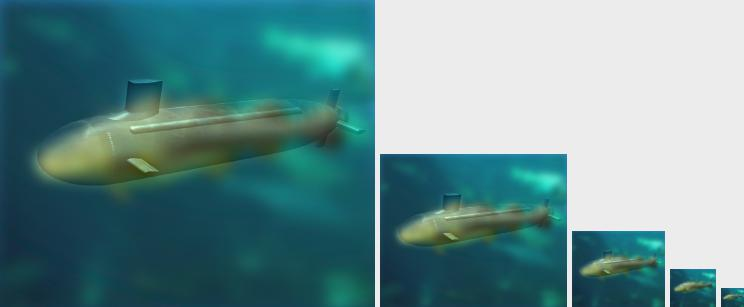
\includegraphics[width=\linewidth]{images/Fish_Sub/hybrid_image_scales_fish_submarine.jpg}
    \caption{Scales}
  \end{subfigure}
  \caption{Different images obtained from proj1.py using a pair of images(Fish-Submarine)}
  \label{fig:coffee3}
\end{figure}

\begin{figure}[h!]
  \centering
  \begin{subfigure}[b]{0.3\linewidth}
    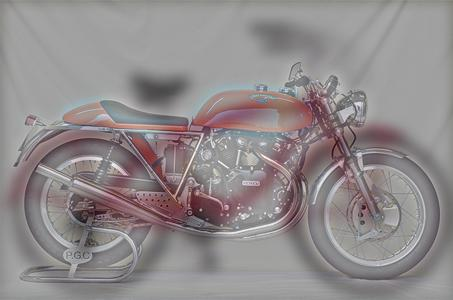
\includegraphics[width=\linewidth, height=3cm]{images/Bicycle_Motorcycle/hybrid_image_bicycle_motorcycle.jpg}
     \caption{Bicycle-Motorcycle}
  \end{subfigure}
  \begin{subfigure}[b]{0.3\linewidth}
    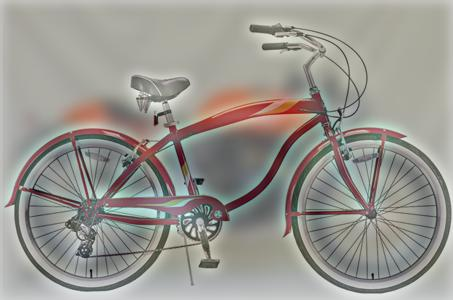
\includegraphics[width=\linewidth, height=3cm]{images/Motorcycle_Bicycle/hybrid_image_motorcycle_bicycle.jpg}
     \caption{Motorcycle-Bicycle}
  \end{subfigure}
  \begin{subfigure}[b]{0.3\linewidth}
    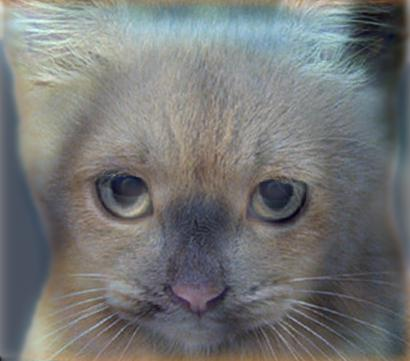
\includegraphics[width=\linewidth, height=3cm]{images/Dog_Cat/hybrid_image_dog_cat.jpg}
    \caption{Dog-Cat}
  \end{subfigure}
  \begin{subfigure}[b]{0.3\linewidth}
    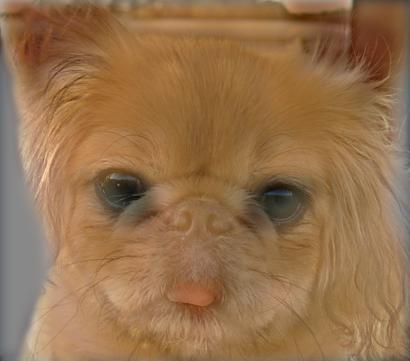
\includegraphics[width=\linewidth, height=3cm]{images/Cat_Dog/hybrid_image_cat_dog.jpg}
    \caption{Cat-Dog}
  \end{subfigure}
  \begin{subfigure}[b]{0.3\linewidth}
    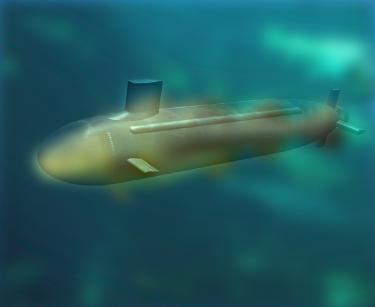
\includegraphics[width=\linewidth, height=3cm]{images/Fish_Sub/hybrid_image_fish_submarine.jpg}
    \caption{Fish-Submarine}
  \end{subfigure}
  \begin{subfigure}[b]{0.3\linewidth}
    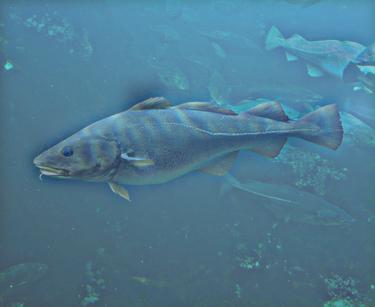
\includegraphics[width=\linewidth, height=3cm]{images/Sub_Fish/hybrid_image_submarine_fish.jpg}
    \caption{Submarine-Fish}
  \end{subfigure}
  \begin{subfigure}[b]{0.3\linewidth}
    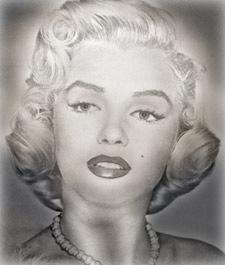
\includegraphics[width=\linewidth, height=3cm]{images/Einstein_Marilyn/hybrid_image_einstein_marilyn.jpg}
    \caption{Einstein-Marilyn}
  \end{subfigure}
  \begin{subfigure}[b]{0.3\linewidth}
    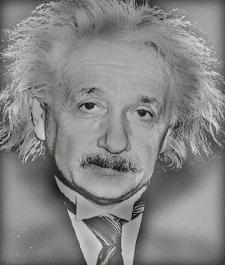
\includegraphics[width=\linewidth, height=3cm]{images/Marilyn_Einstein/hybrid_image_marilyn_einstein.jpg}
    \caption{Marilyn-Einstein}
  \end{subfigure}
  \begin{subfigure}[b]{0.3\linewidth}
    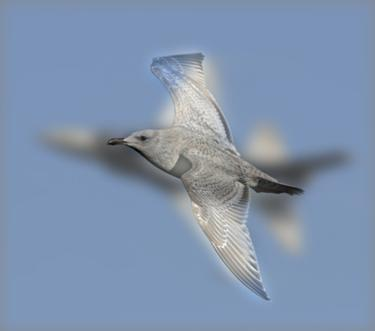
\includegraphics[width=\linewidth, height=3cm]{images/Plane_Bird/hybrid_image_plane_bird.jpg}
    \caption{Plane-Bird}
  \end{subfigure}
  \caption{Different images obtained via proj1.py using a pair of images}
  \label{fig:coffee3}
\end{figure}

Hence we can see that our utility function for filtering is producing correct output
and hence filters are used for a wide variety of applications including edge detection, blurring, sharpening etc. 

Also in case of hybrid images, the combination of low frequencies and high frequencies of two different images
give an effect as if there are two different images 
High frequencies mean an abrupt change in the value that is a sharp change
Low frequencies mean a gradual smooth change. 
It's clear that eyes won't be ablt to detech smooth change from far away so only high frequencies are visible
we have simulated this effect using scales as we scale down the image it gets far from us,
all this is  the essence of this assignment and we have verified all this with programming,maths and input data. 



%------------------------------------------------------------------------


\bibliography{egbib}
\end{document}
